\section{Nutzerumgebung}

\begin{figure}[h]
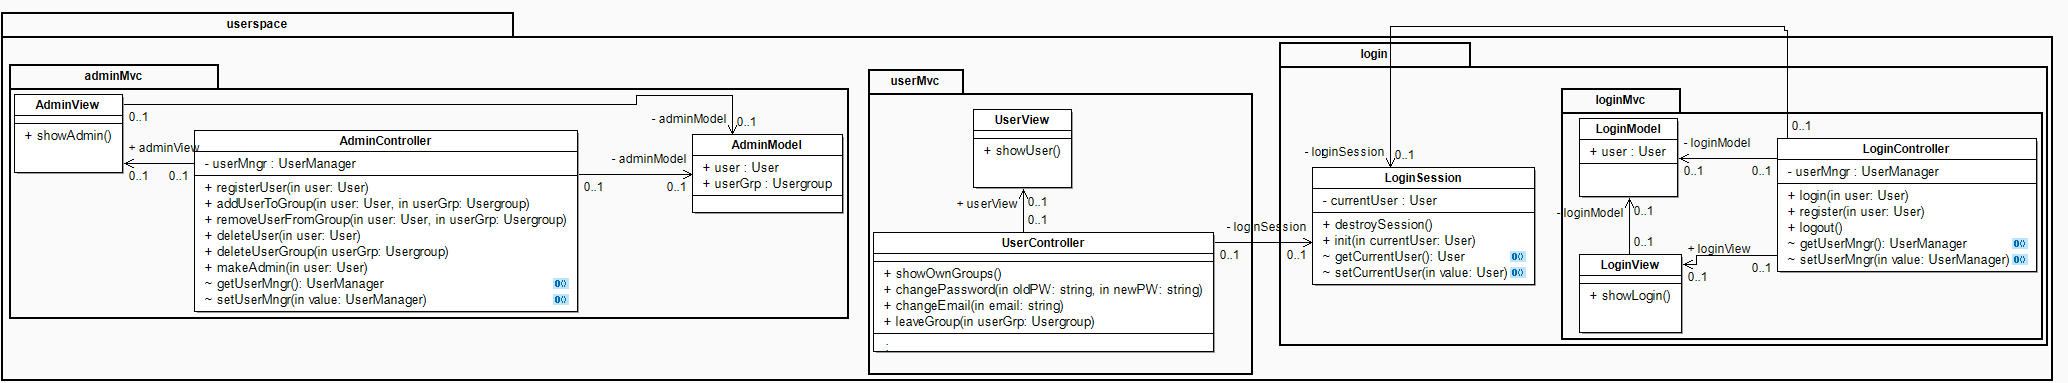
\includegraphics[width=1.0\linewidth]{Grafik/Klassendiagramme/Nutzerumgebung.png}
\caption{Klassen der Nutzerumgebung}
\end{figure}


Die Nutzerumgebung umfasst den Login-Bereich, sowie den Benutzer- und Adminbereich. Die Bereiche sind nach dem Model-View-Controller-Prinzip entworfen. Alle drei Teile werden über eine View-Klasse repräsentiert.
Weiterhin haben alle drei Bereiche jeweils einen Controller. Jeder Controller nimmt die Anfragen der entsprechenden View-Klassen entgegen und 
verarbeitet diese. Zu den Anfragen gehören im Login-Bereich anmelden oder abmelden oder neu registrieren.
Im User-Bereich kann der angemeldete Benutzer seine Angaben  ändern, sowie seine Gruppenzugehörigkeit  - soweit er die Berechtigung hat - bearbeiten.
Ein angemeldeter Administrator kann verschiedene Benutzeroperationen machen, wie Registrieren, Gruppen zuweisen, Benutzer oder -Gruppen löschen sowie  neue Administratoren benennen.
Der Adminbereich hat eine Model-Klasse, in welcher der aktuell bearbeitete Benutzer bzw. die aktuelle bearbeitete Benutzergruppe  zwischengespeichert wird.\\

\noindent Login-Bereich und User-Bereich teilen sich als Model eine Session-Klasse, welche die Informationen zum aktuell angemeldeten Benutzer hält.